\section{Introduction}
\label{sec:intro}
% outline:
% 1. classical method: pre-scanning
% 2. recent efforts: image-based --> typical fashion
% 3. limitation: two fold
% 4. our method: go beyond the SMPL topology, node-based
% 5. overall
% 6. contribution


Animatable human avatar modeling is of great importance in many applications such as content creation and entertainment, and virtual characters have become ubiquitous in our lives with the rise of computer graphics in movies and games. Traditional methods for high-quality human avatar reconstruction are often costly and tedious, due to the difficulties in modeling the complex dynamics of clothes. Besides, they typically presume the availability of a subject-specific template~\cite{habermann2021realtimeDDC} and its accurate registration to the input frames~\cite{timur2021driving_signal,Xiang2021ModelingClothing}, which are difficult to acquire in practice.

With the rapid development in computer vision in the past ten years, researchers have started to explore the possibility of automatic human avatar reconstruction without pre-scanning efforts. Pioneer studies deformed a statistical human body template (e.g., SMPL \cite{loper2015smpl}) to model the clothed human geometry and appearance \cite{alldieck2018videoavatar,alldieck2018videoavatar_detailed,alldieck19octopus}. Neural texture maps and image-to-image networks are later adopted to achieve photo-realistic rendering \cite{Liu2018Neural,liu2020NeuralHumanRendering,Shysheya2019TNR,raj2020anr}. Recently, neural radiance representations, which implicitly encode shape and appearance using neural networks, are also applied in pursuit of higher-fidelity results \cite{peng2021animatable_nerf,noguchi2021narf,neural_actors}. These methods typically define the radiance field in a canonical pose, and warp it to live poses using linear blending skinning (LBS) under the guidance of the SMPL surface. 


\begin{figure}
    \centering
    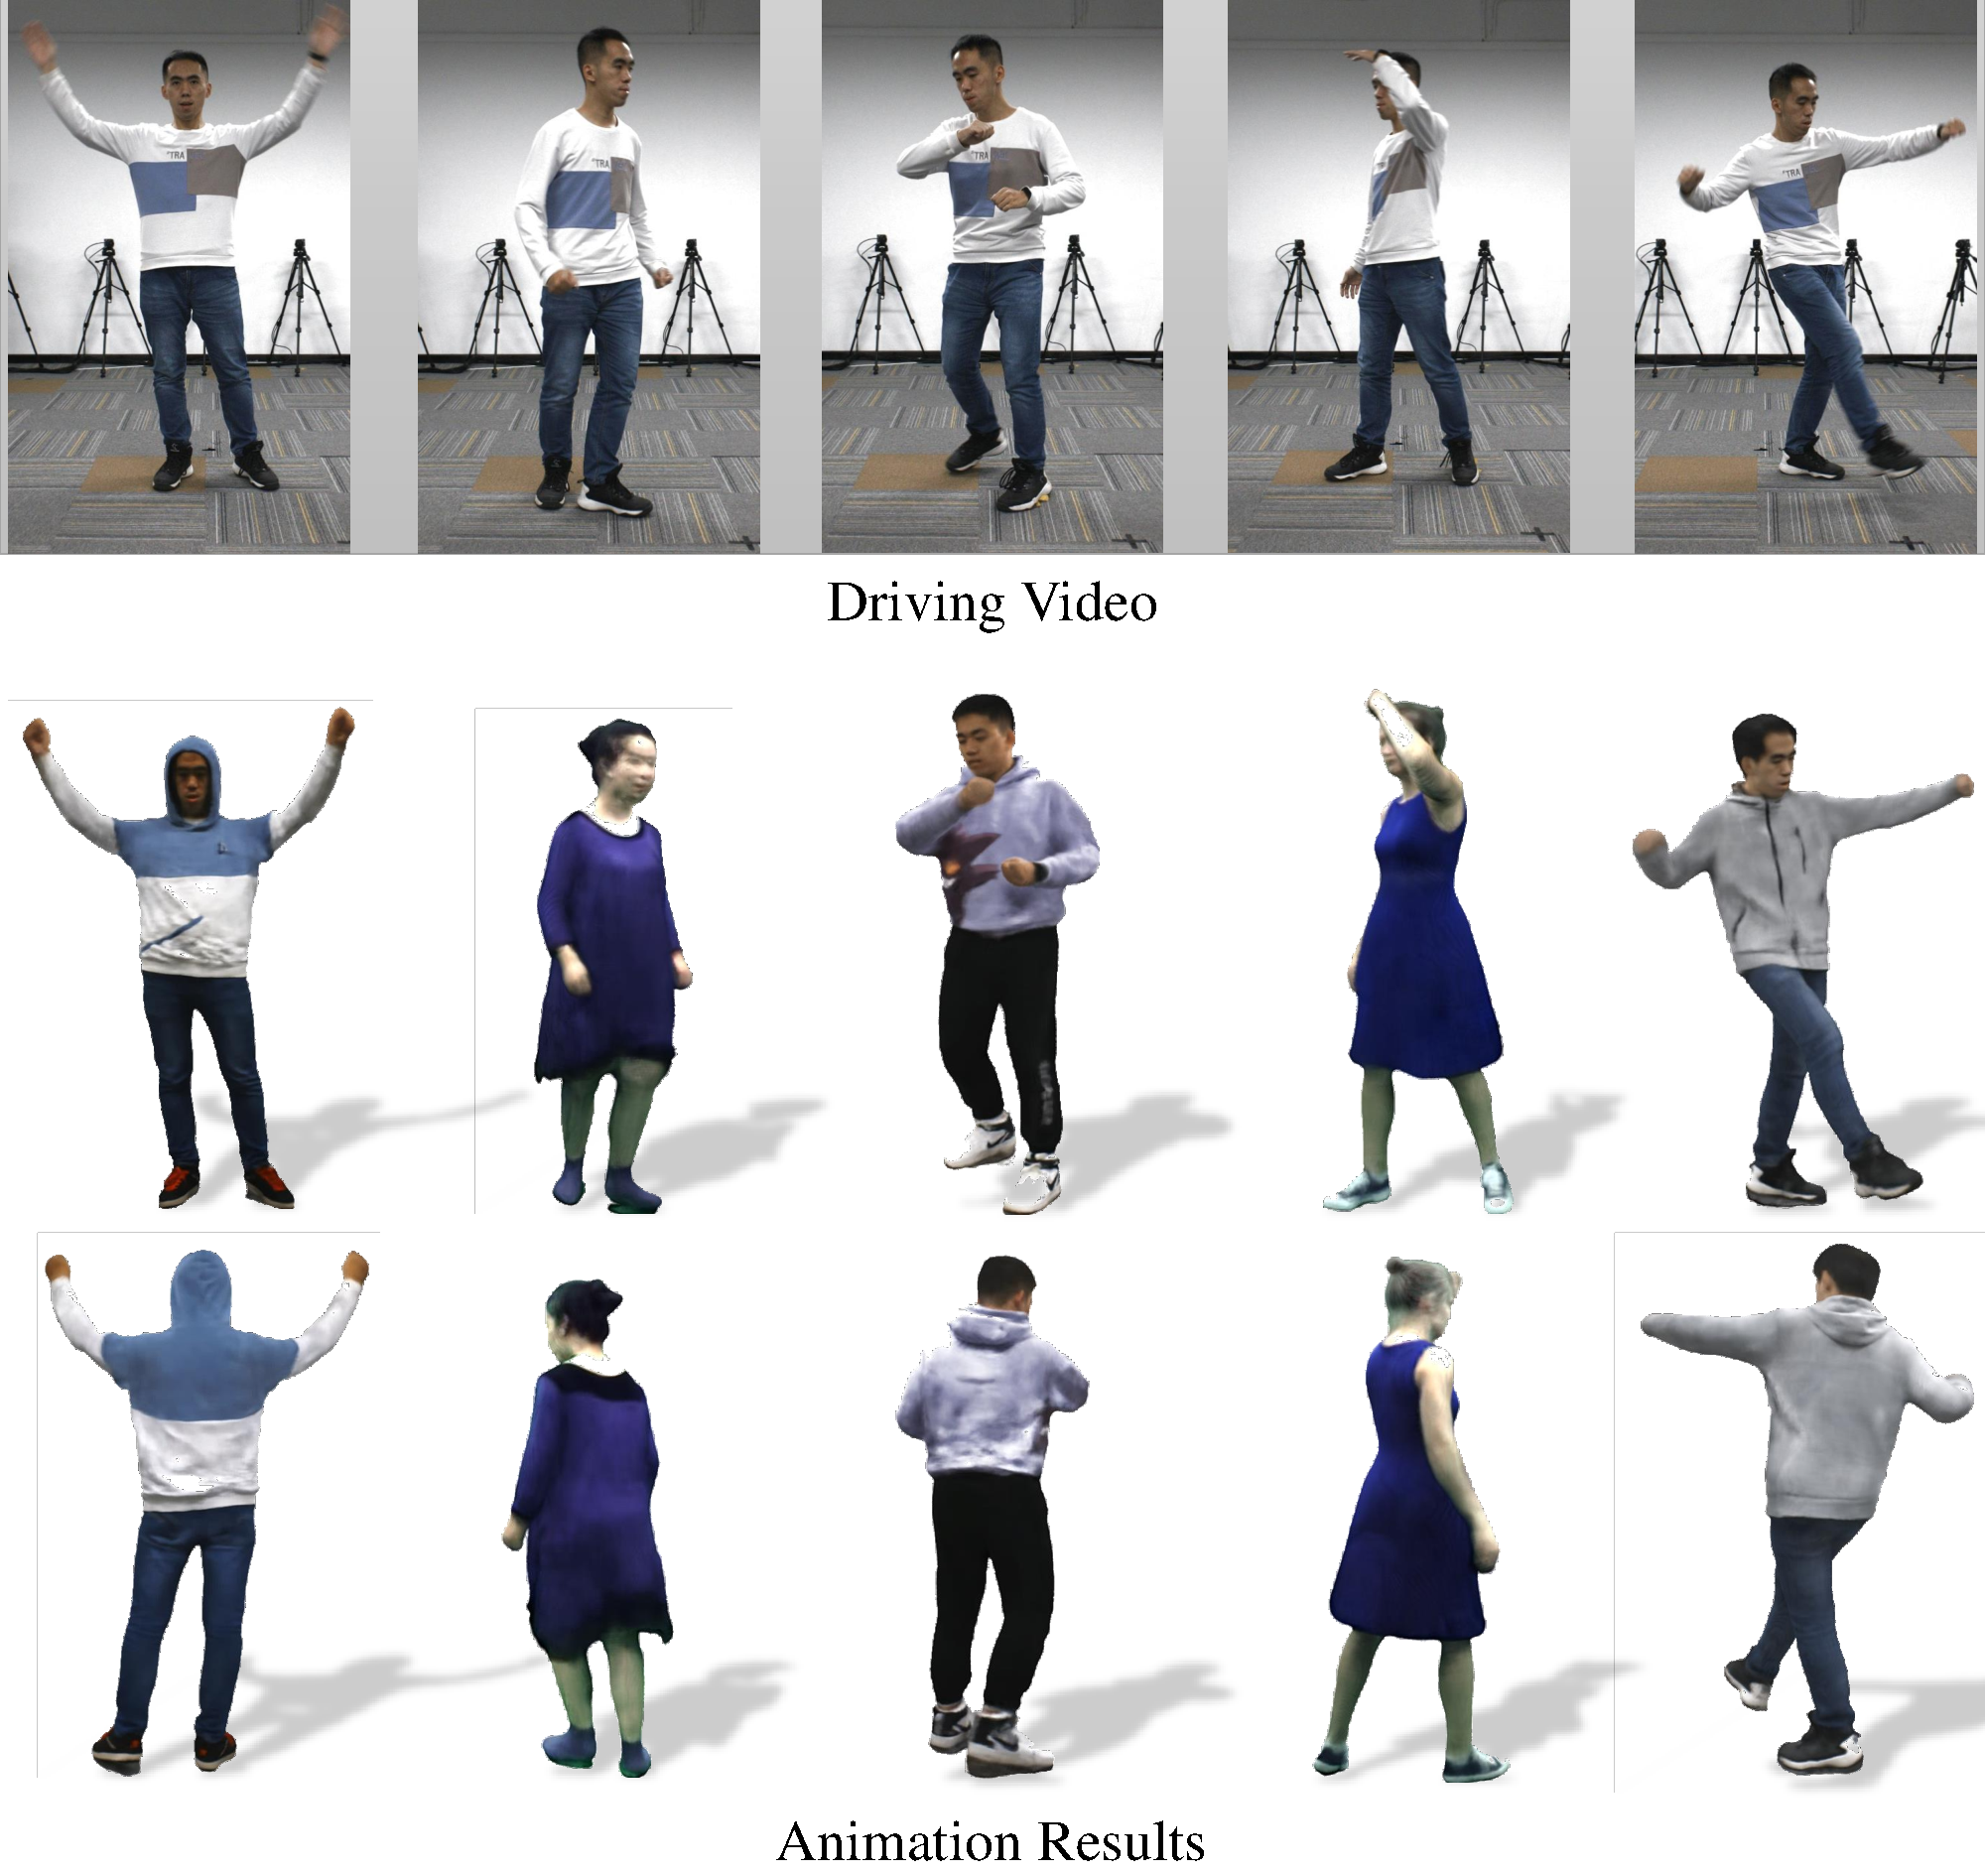
\includegraphics[width=1.0\linewidth]{teaser}
    \caption{\textbf{Example results produced by our method.} Our method can learn animatable human avatars with various cloth topologies and realistic dynamic details. Top row: driving video, from which the animation poses are extracted. Bottom two rows: animation results rendered from the front and the back view.  }
    \label{fig:teaser}
\end{figure}


Despite the differences in the representations inside the aforementioned approaches, we find that there is one thing in common: they all heavily rely on the skeleton or the surface of SMPL model for cloth motion modeling. This is apparent in methods based on the SMPL topology, either using traditional texture maps \cite{alldieck2018videoavatar,alldieck2018videoavatar_detailed,alldieck19octopus} or neural textures \cite{Liu2018Neural,liu2020NeuralHumanRendering,Shysheya2019TNR,raj2020anr}. Even in state-of-the-art methods based on implicit fields \cite{peng2021animatable_nerf,noguchi2021narf,neural_actors}, researchers still assumed that skin motions can be propagated to approximate the cloth deformations, which, unfortunately, only holds for tight-fitting clothes. 
When applying these methods to loose clothes, articulation motions based on solely body joints cannot express the complete information about the wrinkles and non-rigid deformations. Some methods learned to directly regress cloth deformations from body pose configurations~\cite{neural_actors}; however, the complexity gap between body poses and cloth details results in a one-to-many mapping problem, leading to under-fitting issues where the network learns averaged, blurry appearance. 
Suffering from this fatal limitation, no methods have demonstrated animatable human characters wearing skirts or dresses so far. 

To overcome this limitation and fill the void, we propose a new representation for clothed human characters. Our representation is built upon neural radiance fields~\cite{mildenhall2020nerf}, or NeRF in short, for its excellent performance in learning the appearance of static scenes. To extend NeRF for dynamic character modeling, we break a global NeRF into a set of \emph{structured local radiance fields}, which are attached to the pre-defined nodes on the SMPL model. Each local radiance field is responsible for representing the shape and appearance in the local space around its corresponding node. The local radiance fields can be driven by the body skeleton, while having their own residual movements to represent the non-rigid deformation of garments. Furthermore, each radiance field is conditioned on a dynamic detail embedding, which encodes the high-frequency dynamic details that cannot be modeled via node translation. In this way, our representation decomposes the cloth deformations in a coarse-to-fine manner: the coarsest level is the skeleton motion, the middle level is the residual movements of the local radiance fields, and the finest level is the time-varying details inside each radiance field. 

However, employing such a representation for avatar modeling is not straight-forward as the node-related variables (\textit{i.e.}, the node residual translations and the dynamic detail embeddings) are difficult to acquire in practice. 
Although we can obtain these variables for training frames through naive optimization with image evidence, it remains unclear how to compute them for unseen poses. 
Alternatively, one can train a network that directly regresses these variables from body poses, but this will result into the aforementioned under-fitting issues due to information deficiency~\cite{timur2021driving_signal}. 
% the node-related variables (\textit{i.e.}, the residual translations and dynamic detail embeddings) are both difficult to acquire in practice. 
% Our ultimate goal is to build a clothed human avatar that can not only explain the observation of training images but also generate the images of unseen poses. 
% This requires us to achieve a balance between data fitting and generalization. 
%To fulfill this goal, we need to 1) find the optimal node translations and detail embeddings for training frames, and 2) generate plausible values for these variables given unseen poses. 
In order to achieve a balance between data fitting and generalization, we draw inspiration from \cite{timur2021driving_signal} and learn the node-related variables in a conditional generative latent space. Specifically, we introduce a tiny conditional variational auto-encoder (cVAE)~\cite{Sohn2015cvae} for each local radiance field. 
Conditioned on the pose parameters, the cVAE decoders convert the latent bottlenecks into node-related variables. For the input of the cVAE encoder, we find that the time stamp~\cite{Pumarola20arxiv_D_NeRF,Xian20arxiv_stnif,Gao-freeviewvideo} is an effective option, because it is simple, distinguishable, and naturally guarantees the temporal smoothness of the node-related variables thanks to the low-frequency bias in MLPs~\cite{tancik2020fourfeat}. 
Intuitively, the time stamp is provided as an auxiliary input to help our network distinguish similar poses at different frames, while the VAE property can push the latent space to be uninformative, thereby encouraging the network to mainly rely on pose conditions when inferring node-related variables. 
With all of these building blocks, our network can be trained in an end-to-end manner, eventually producing a realistic dynamic human avatar. 


% find a interesting option: the time stamp, which is simple, distinguishable, and naturally guarantees the temporal smoothness of the unknown variables thanks to the low-frequency bias in MLP~\cite{tancik2020fourfeat}. 

% However, employing such a representation is not straight-forward: unlike body poses, the node residual translation and dynamic detail embeddings are both difficult to acquire in practice, especially for . 
% Our ultimate goal is to build a clothed human avatar that can: 1) explain the observation of training image, and 2) generate the image of unseen poses. To fulfill this goal, we need to find a way of 


% To address this challenge, we draw inspiration from \cite{timur2021driving_signal} and model these variables in a conditional generative latent space. Specifically, we design a tiny conditional variational auto-encoder (cVAE)~\cite{Sohn2015cvae} for each local radiance field. 

% unsupervised

% generative latent space

% time instant as the encoder input

% ~\cite{Pumarola20arxiv_D_NeRF,Xian20arxiv_stnif,Gao-freeviewvideo}

Overall, our proposed method offers the new ability to automatically create an animatable human character with general, dynamic garments. This is achieved by using only RGB videos, without any pre-scanning efforts. Compared to methods that heavily depend on the topology of a naked human body template, our approach is powerful yet general in terms of both appearance learning and motion modeling, and able to generate realistic dynamic details. To the best of our knowledge, our method is the first one that demonstrates automatic human avatar creation for dresses. Experiments prove that our method outperforms state-of-the-art approaches qualitatively and quantitatively. 
% These advantages are enabled by the following technical contributions:
% To enable the above advantages, we make the following technical contributions in this paper:
% To summarize, we make the following technical contributions in this paper:
% \begin{itemize}[leftmargin=*]
% \setlength{\itemsep}{0pt}
% \setlength{\parsep}{0pt}
% \setlength{\parskip}{0pt}
% \vspace{-0.2cm}
%     \item We propose structured local radianc fields (Sec. \ref{sec:overview}) as a new representation for high-quality avatar learning from RGB videos. Our representation is powerful yet general in terms of both appearance learning and motion modeling, showing superiority over existing methods that heavily depends on the topology of a naked body template. 
%     \item To handle the complex mapping from body pose to cloth details, we  (Sec. \ref{sec:method}).  
%     \item To the best of our knowledge, our method is the first one that demonstrates automatic human avatar construction for loose clothes dresses (Sec. \ref{sec:experiments}). This is achieved by using only RGB inputs, without any pre-scanning efforts. Extensive experiments prove that our method outperforms state-of-the-art methods qualitatively and quantitatively. 
% \vspace{-0.2cm}
% \end{itemize}
